\section{Analysis}
\subsection{Problem Defenition}
This project aims to produce a user-friendly means to interact with the SpaceTraders API, an online space trading game that uses http requests to communicate with the server and manage a fleet of ships, however that lacks a frontend client for users to interact with. The core gameplay loop revolves around accepting loans, and performing mining operations to gather the required resources to repay those loans. Credits can then be used to improve your fleet and in turn, increase one's mining capacity – allowing larger loans to be taken for more credits.

To play Space Traders you must first register yourself a callsign e.g. (L3O, TR4D3R etc..) which identifies an agent. Contracts, ships, and credits are all associated with an agent identity. The Space Traders universe is composed of systems and waypoints. Waypoints are locations within a system such as a planet, moon or asteroid, and consist of a type, x-y coordinates, and set of features such as a shipyard or marketplace. Ships can navigate between waypoints or warp between systems. An agent earns credits by taking contracts with a deadline and requirements for completion e.g. (deliver "205 IRON\_ORE" to destination: "X1-QT13-H53" by "2024-03-15T12:04:25.707Z"). 

To complete a mining contract, you must locate an asteroid containing the required ore, and send your purchased mining droid to mine the resource. Cargo can then be sold at marketplaces to earn credits and offload cargo, with variable market rates for each resource depending on the volume being traded; which affects both the stability and magnitude of the market price. 

Since SpaceTraders lacks a frontend for users to interact with, actions are performed via http requests sent to the Space Traders server. For example, this request to navigate to the waypoint X1-QT13-H53:
\begin{lstlisting}
curl --request POST \
 --url 'https://api.spacetraders.io/v2/my/ships/L30_DE-1/navigate' \
 --header 'Authorization: Bearer eyJ[...]pQw' \
 --header 'Content-Type: application/json' \
 --data '{
    "waypointSymbol": "X1-QT13-H53"
   }'
\end{lstlisting}

\subsection{Programming Language}
The first decision to make regarding to this project is that of programming language – more specifically a choice between two stable, statically typed languages with strong module support and asynchronous runtimes. Go and Rust. The former (renowned for its simplicity and concurrency) would offer an expediated development cycle with an extensive standard library. Rust, however, offers memory safety, performance and a strict typing system – enforcing good programming practices. In addition to a superior multiplatform bundler for distributing the program as a single binary without dependencies. Furthermore, Rust has a more mature and documented ecosystem for Terminal User Interfaces (TUI) and Command Line Interfaces (CLI) – which I intend to explore as a means for the user to interact with the API. Below is the same program demonstrating registration with the SpaceTraders API written in Rust and Go respectively to illustrate their differences. 

\subsubsection{Prototyping}
\begin{lstlisting}[language=C]
use std::collections::HashMap;
use reqwest::{Client, Error};

async fn register() -> Result<String, Error> {
    let client = Client::new();

    let agent = HashMap::from([
        ("symbol", "L30_DESILVA"), 
        ("faction", "COSMIC")
    ]);

    let res = client
        .post("https://api.spacetraders.io/v2/register")
        .header("Content-Type", "application/json")
        .json(&agent)
        .send()
        .await?
        .json::<serde_json::Value>()
        .await?;

    if let Some(error) = res.get("error") {
        println!("{}", error["message"])
    } else {
        println!("Congratulations, {}. You have been 
            registered. Please note your token.", 
            res["data"]["agent"]["symbol"]);
        println!("{}", res["data"]["token"]);
    }

    Ok(res["data"]["token"].to_string());
}

#[tokio::main]
async fn main() {
    let _ = register().await.unwrap();
}

\end{lstlisting}

\begin{lstlisting}
$ http_prototype git:(master): cargo run
    Compiling http_prototype v0.1.0 
      Finished dev [unoptimized] target(s) in 0.51s
      Running `target/debug/http_prototype`

Congratulations, "L30_DESILVA". You have been registered.
Please note your token:
"eyJhbGciO[...]QhEdECLg"

$ http_prototype git:(master): cargo run
    Finished dev [unoptimized] target(s) in 0.07s
     Running `target/debug/http_prototype`

"Cannot register agent. Agent symbol L30_DESILVA has already been claimed." 

\end{lstlisting}

The equivalent Go code, due to its simplicity, can be tedious and lengthy to write. 

\begin{lstlisting}[language=C]
package main

import (
	"bytes"
	"encoding/json"
	"fmt"
	"net/http"
)

type Register struct {
    Data map[string]interface{}
    Error map[string]interface{}
}

func main() {
    body, err := json.Marshal(map[string]string{
        "symbol": "TRUCKER",
	 "faction": "COSMIC",
    }) 

    if err != nil {
        panic(err)
    }

    req, err := http.NewRequest(
        "POST",       
        "https://api.spacetraders.io/v2/register", 
        bytes.NewBuffer(body)
    )

    if err != nil {
        panic(err)
    }

    req.Header.Add("Content-Type", "application/json")
    client := &http.Client{}
    res, err := client.Do(req)
    if err != nil {
        panic(err);
    }

    defer res.Body.Close()

    data := Register{}
    err = json.NewDecoder(res.Body).Decode(&data)
    if err != nil {
        panic(err)
    }

    if len(data.Error) != 0 {
        fmt.Println(data.Error["message"])
    } else {
        var agent map[string]interface{}
        agentJson, err := json.Marshal(data.Data);
        if err != nil {
            panic(err)
        }

        err = json.Unmarshal(agentJson, &agent);
        if err != nil {
            panic(err)
        }

        fmt.Printf("Congratulations, You've been successfully registered. Please note your access token:\n")
        fmt.Println(agent["token"])
    }
}
\end{lstlisting}

Due to its stability, performance, security and mature, centralised ecosystem I will use rust for this project. Although Rust’s somewhat convoluted approach to asynchronous programming will require careful design considerations as to not introduce bugs. And it's combination of a restrictive borrow checker and strict compiler enforces good programming practices and memory safety, with verbose handling of all potential errors mitigting the risk of crashes and ensuring programs are always stable, performant and reliable. 

\subsection{API}
A web API (Application Programming Interface) is a set of standard protocols to interact with a web server. The Space Traders API offers HTTP end-points with which programs can access, and in turn: play the open universe trading game. Actions are performed via http requests to the Space Traders server, and such actions can range from locating all available shipyards in a system (\textcite{spacetraders}):
\begin{lstlisting}
curl 'https://api.spacetraders.io/v2/systems/:systemSymbol/waypoints?traits=SHIPYARD' --header 'Authorization: Bearer INSERT\_TOKEN\_HERE'
\end{lstlisting}
To selling ship cargo:

\begin{lstlisting}
curl --request POST \
 --url 'https://api.spacetraders.io/v2/my/ships/:miningShipSymbol/sell'
 --header 'Authorization: Bearer INSERT_TOKEN_HERE' \
 --header 'Content-Type: application/json' \
 --data '{
    "symbol": "IRON_ORE",
    "units": "100"
   }'
\end{lstlisting}

However, there are 2 versions of the SpaceTraders API in production, the complete V1, and the alpha V2 release. The former is a simpler system, more mature, and has a wider variety of existing frontend clients to learn from. Yet lacks much of the functionality of the second release.  Whereas V2 consists of a larger universe, a wider breadth of features, and comprehensive documentation. (\textcite{spacetraders}) Thus, my project will utilise the V2 API specification albeit hesitant of potential bugs due to the alpha nature of its release. 

\subsection{Existing Systems}
There are various existing frontends that use either a command line interface (CLI), or a graphical user interface (GUI) to interract with the SpaceTraders API. A command line interface (as illustrated below) allows for expediated development, however can appear confusing, intimidating, and untintuitive without experience, wheras a GUI whilst visually intuitive, offers less flexibility and a slower development cycle. A common thread between all clients is the manner in which systems distill the complex http queries into a simpler interface when interacting with the server.
\bigskip

\shadowbox{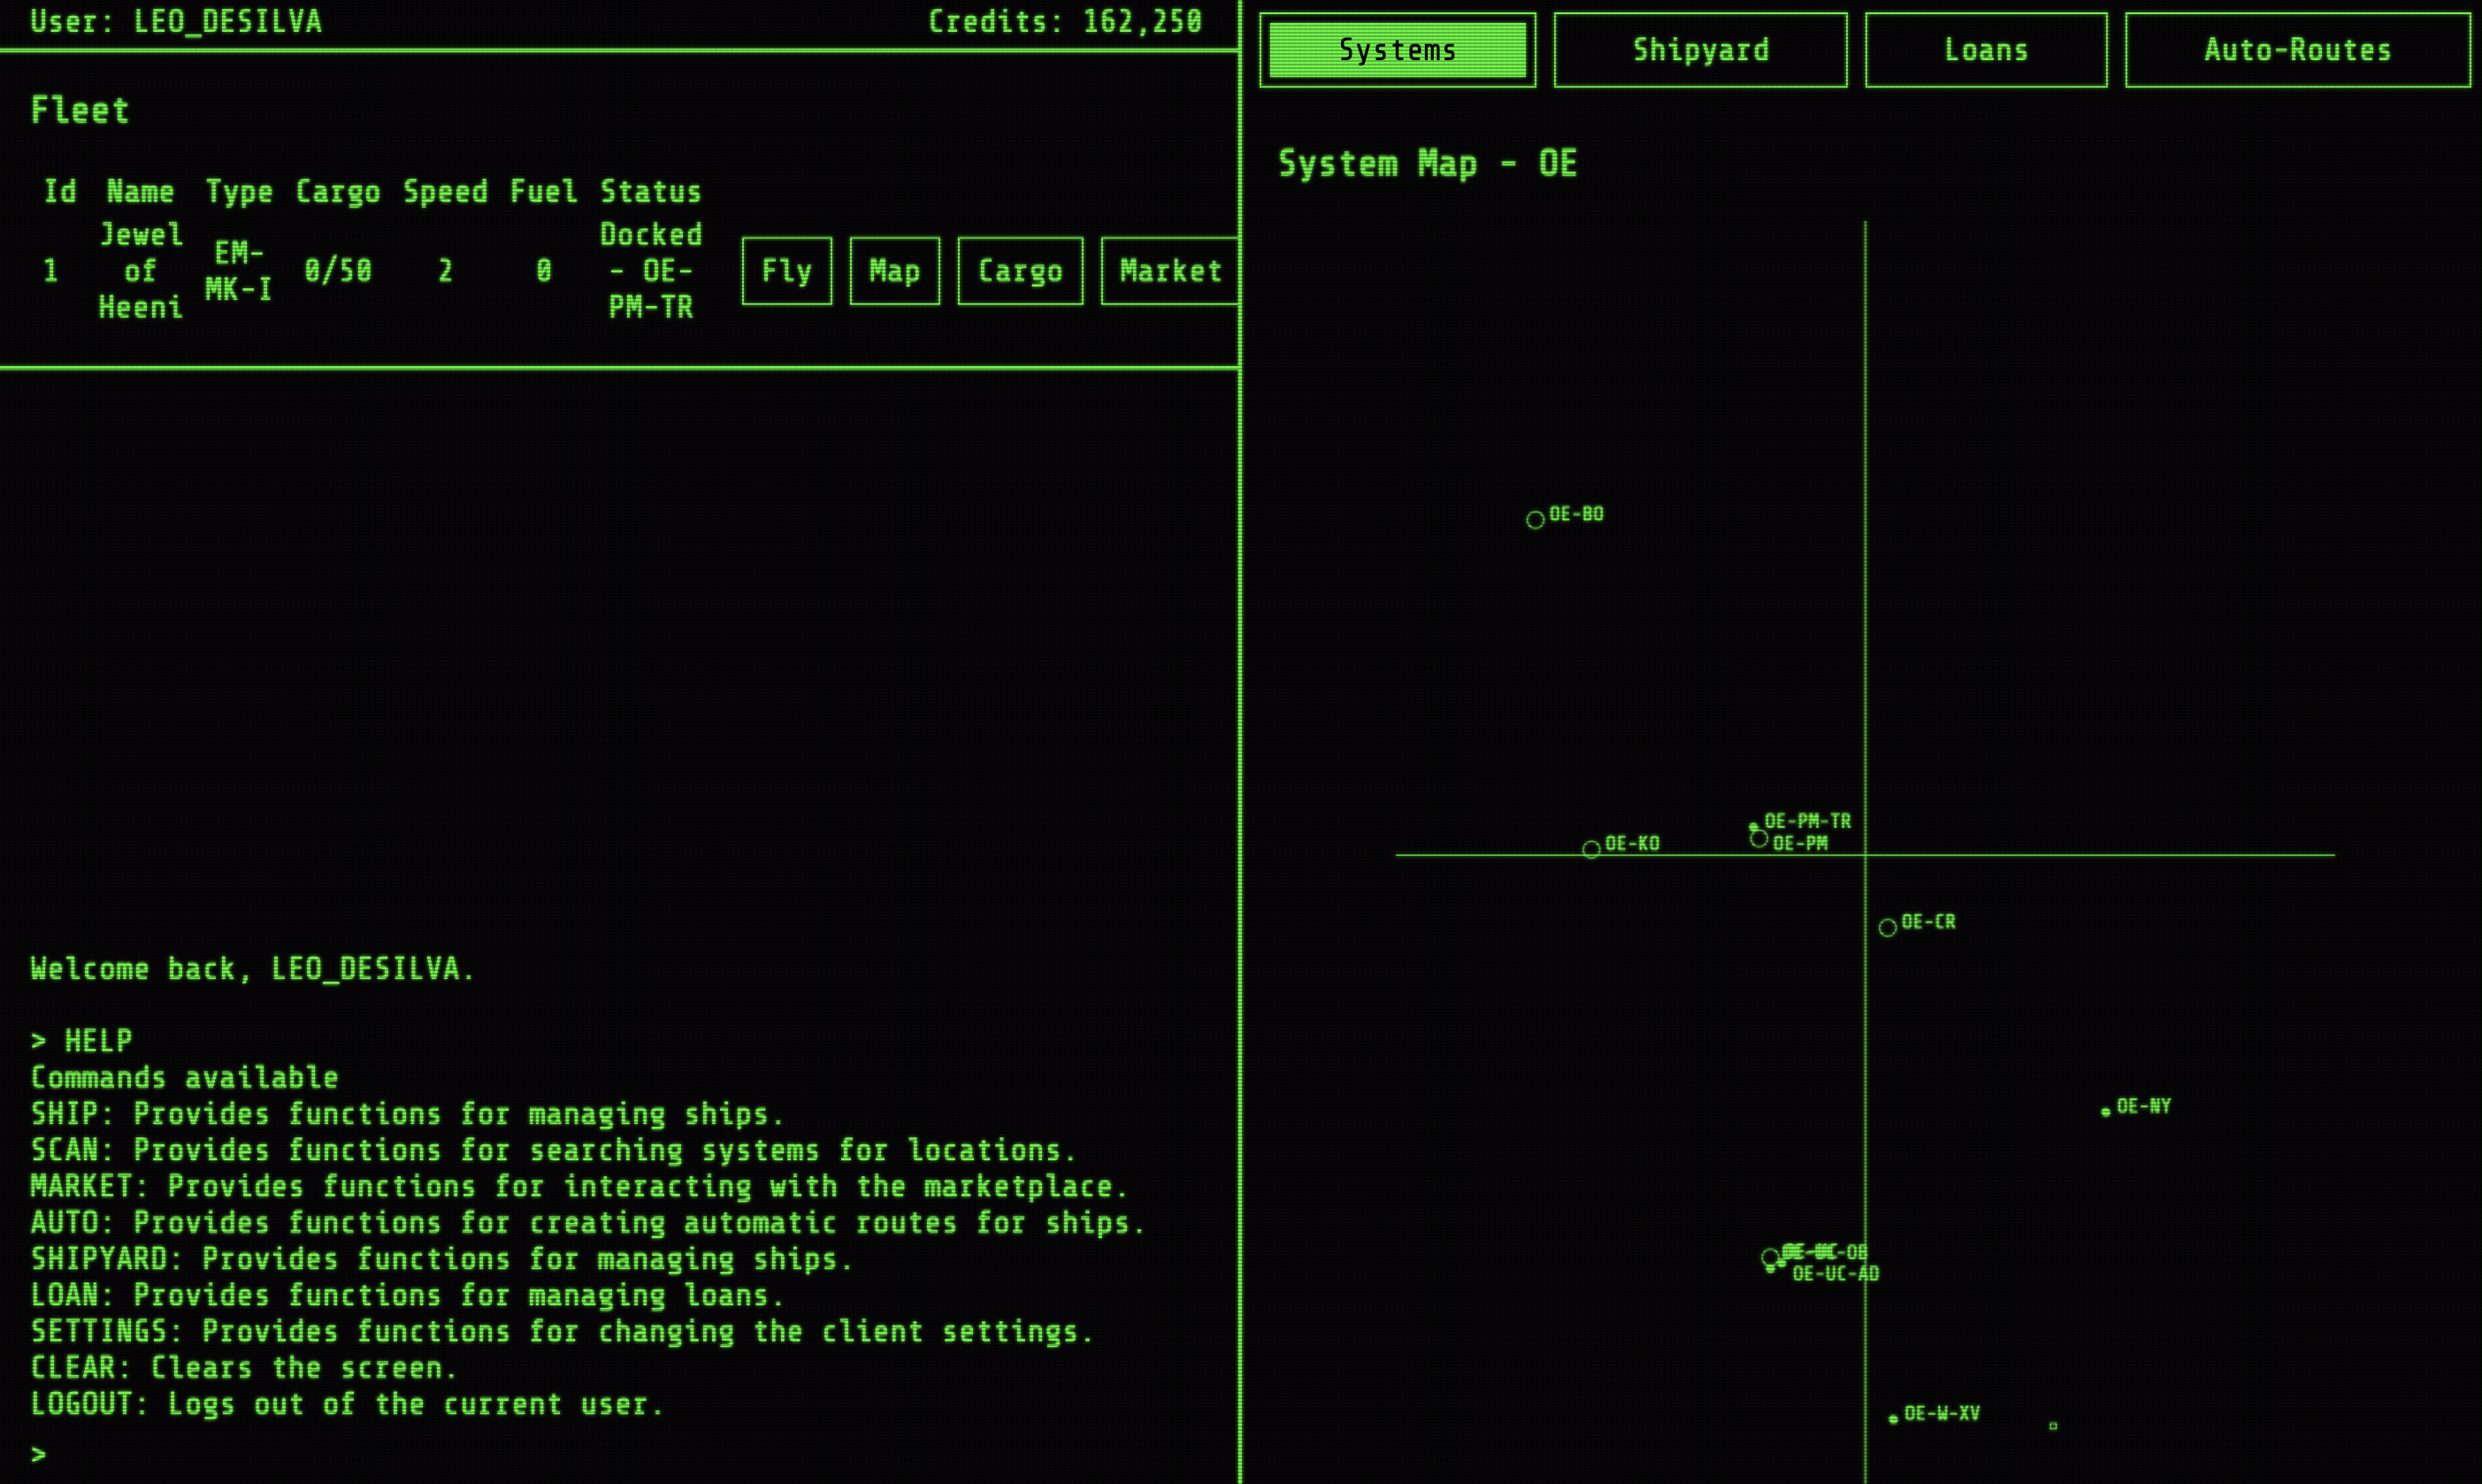
\includegraphics[width=11cm]{trade-commander.png}}

Trade Commander (\textcite{tradecommander}) is a CLI client for the SpaceTraders API that uses a split screen approach where commands are input in the console on the left and their output shown graphically through the display on the right. Trade Commander thus merges the flexibility of textual interfaces with the intuitiveness of a GUI. It offers a dashboard layout where commonly relevant information can be accessed at a glance: such as ones fleet, star map, owed loans, and trade market. This has the advantage of being efficient to use, however comprises a considerable learning curve when initially getting started with Space Traders.  

\bigskip
\shadowbox{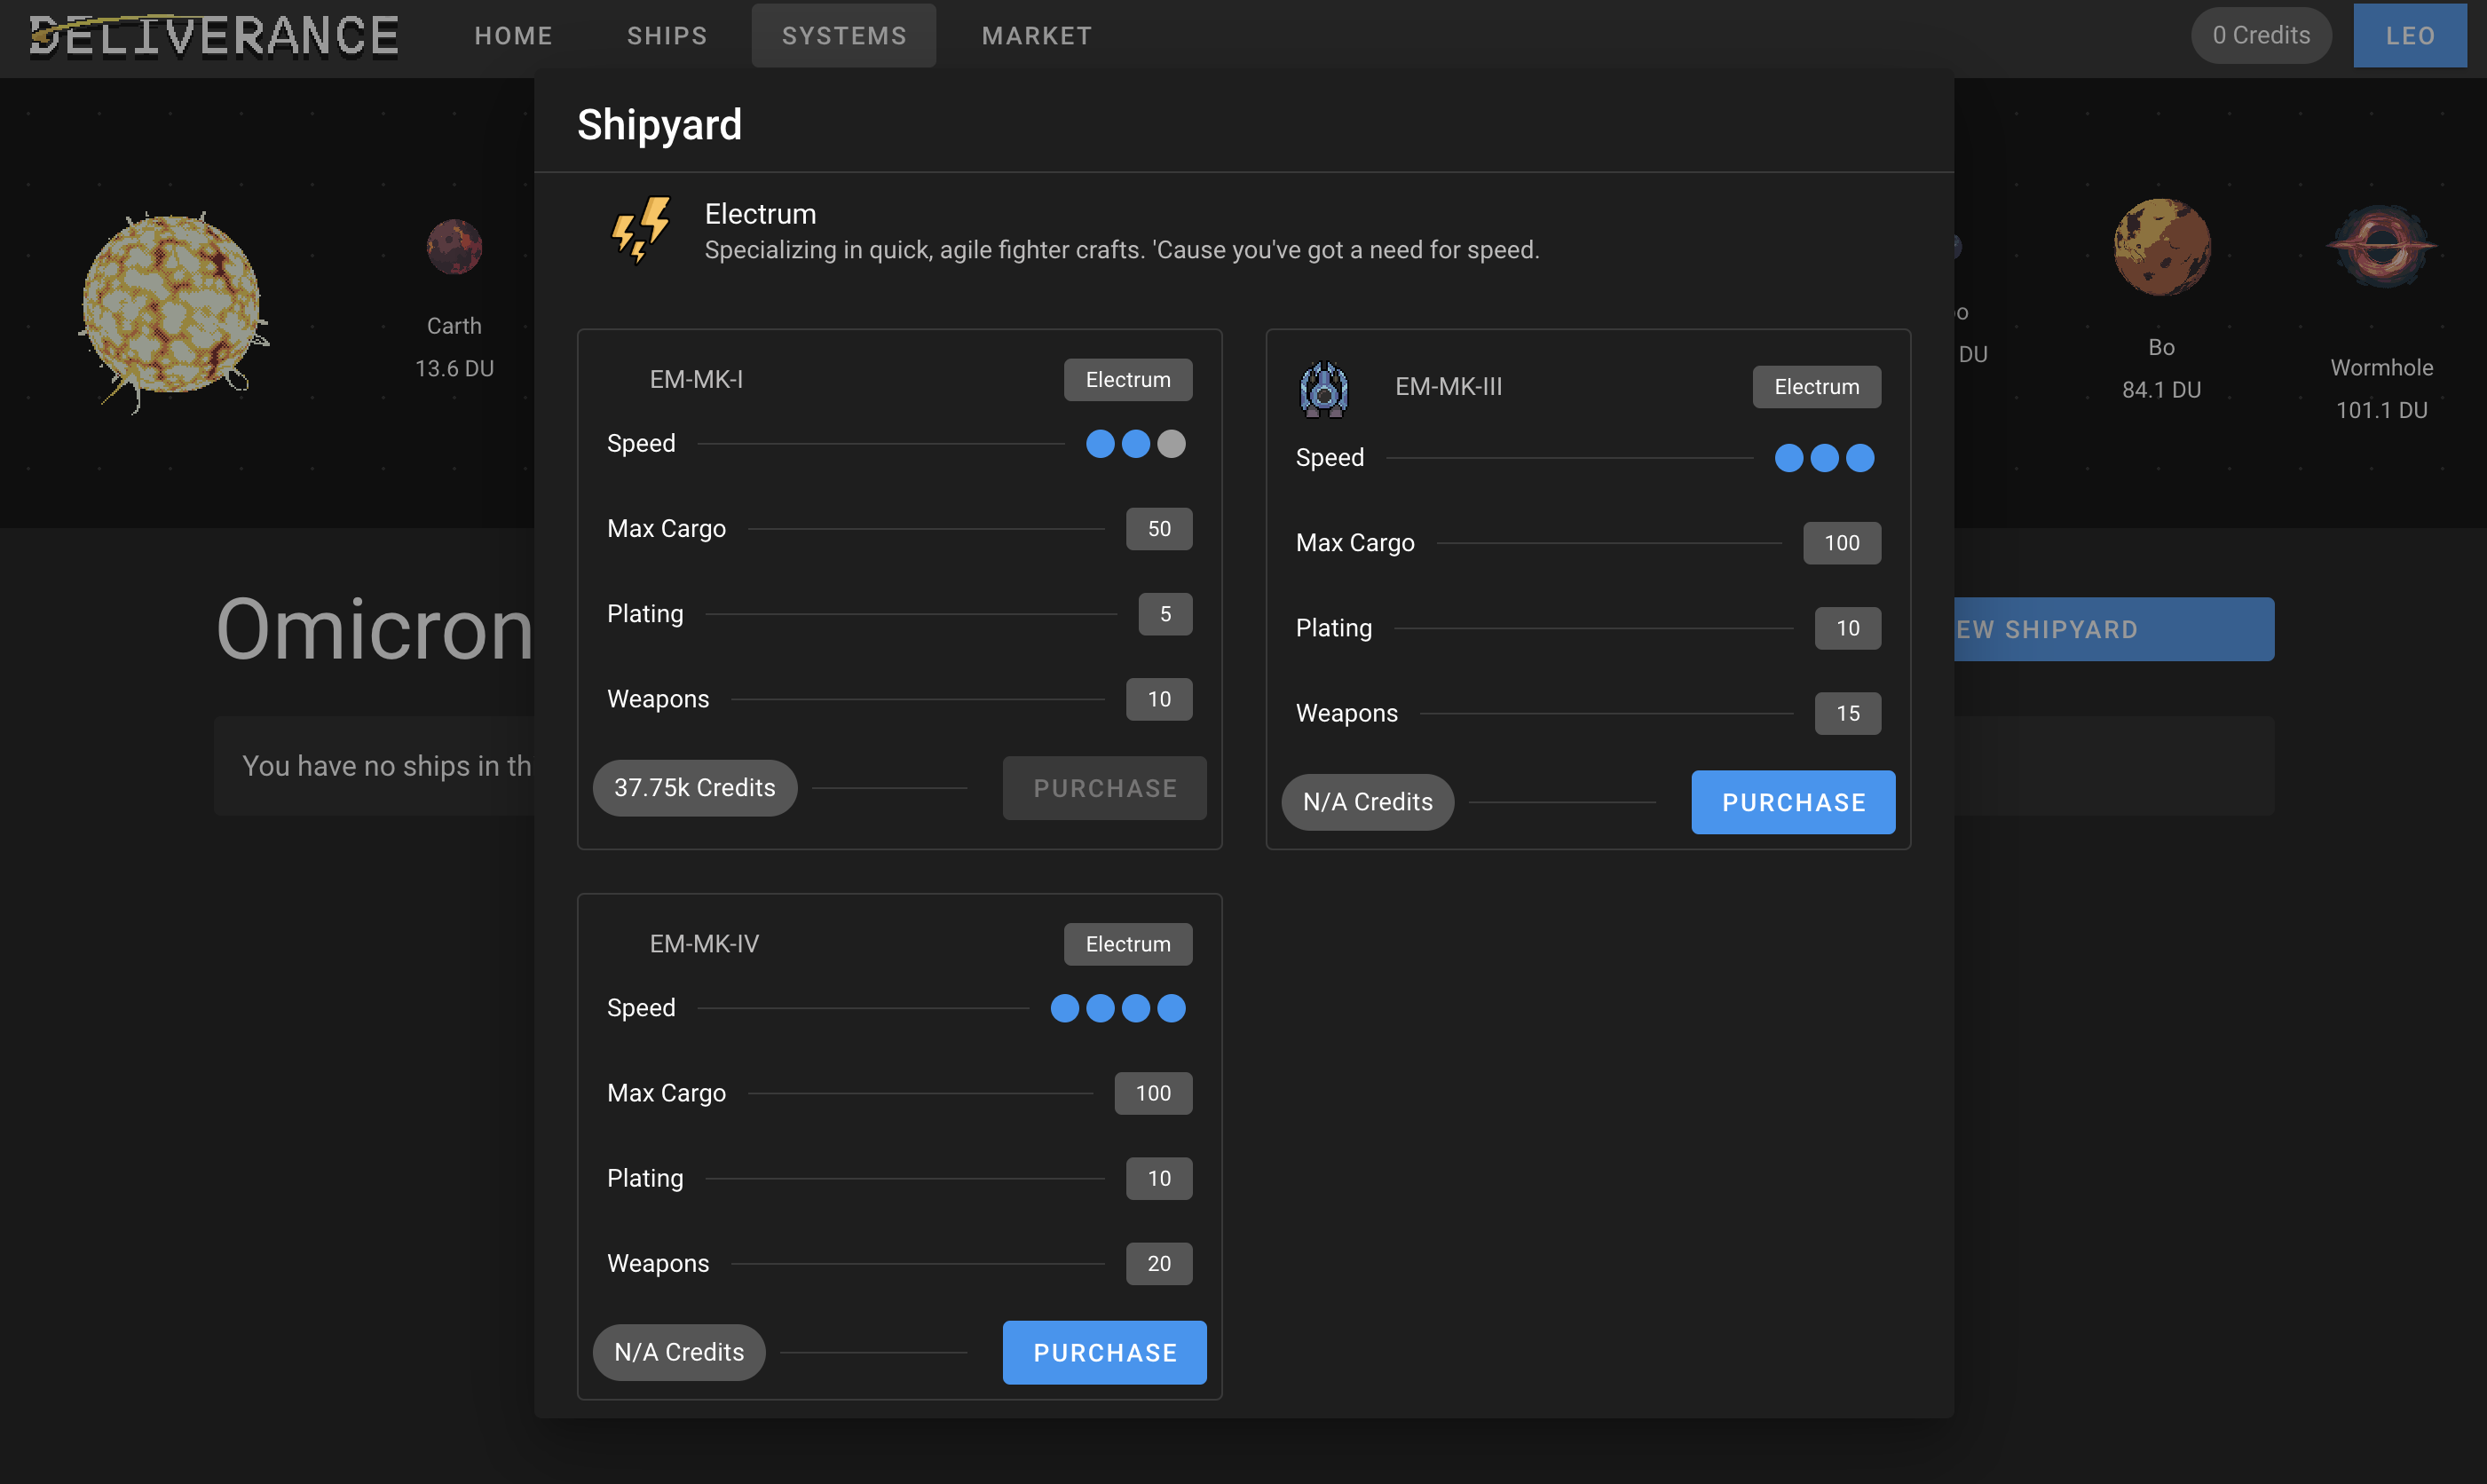
\includegraphics[width=11cm]{deliverance.png}}

Deliverance (\textcite{deliverance}) took a different approach, opting for a graphical UI, synthesising the http requests required to interact with the API into a series of menus and buttons that are intuitive to work with. Stumblinbear has organised the available operations into 4 categories: Home, Ships, Systems, and Market. This has the advantage of being comparatively easy to work with, however will slow down development due to the resources needed to create a graphical interface and limits the flexibility of the system when adding new functionality.

In conclusion, I will look at approaching my frontend similarly to that of Trade Commander, with an interspersion of textual and graphical elements, creating a more 'retro' aesthetic that suits the nature of the game. 

\subsection{Client Proposal}
The set of features I will propose to my client is as following:
\begin{enumerate}
    \item A Terminal User Interface (TUI) comprising of a command line and graphical interface.
    \item The ability to register or login to an account using an access token.
    \item The ability to purchase ships and manage one's fleet.
    \item The ability to take out and repay loans.
    \item The ability to manage one's mining operations.
    \item The ability to visually display a map of the star system.
    \item The ability to query \& display data logically \textit{(e.g. sort available ships by price)}
\end{enumerate}

My system will use integrate aspects of both a CLI and GUI. The console permits the flexibility of input that is limited by a GUI, and the graphical interface can display the results of such commands or other relevant information to the user, including but not limited too: a map of the star system, the progress of ongoing mining operations, any pending loans etc... My system will include means of querying data from the API which can be sorted and displayed according to the user's requirements, such as ordering loans by their reward, or displaying all unsold ships in the system. 

\subsubsection{Client Interview}
I will interview my client about their experience playing Space Traders, and gather their thoughts on the frontends they have used. Here are the questions I intend to ask:
\begin{enumerate}
    \item Have you ever played a game of Space Traders?
    \item Which features of your client(s) did you like?
    \item Which features of your client(s) did you dislike?
    \item Which part of the game did you find the most difficult to understand? And what could have helped you understand it better?
    \item Did you find a graphical interface improved your understanding of the game?
    \item Would you have found a tutorial system beneficial to your enjoyment when first starting out with Space Traders? 
\end{enumerate}
